\section{Autobidding with Regenerating Budgets}
\label{sec:exp4a_results}

Experiments~1--3 studied tabular and bandit learners that bid directly from value estimates. Modern ad exchanges, however, rely on budget-constrained pacing agents that modulate bids across campaigns. We now test whether the dominance of market thickness persists in this qualitatively different setting. Experiment~4a shifts from tabular learners to dual-based autobidding agents operating under regenerating budget constraints. Each of $N$ advertisers bids in $D = 100$ episodes of $T = 1{,}000$ auctions, with budgets resetting between episodes while dual variables warm-start, mimicking daily budget cycles in ad exchanges. Valuations are drawn from bidder-specific log-normal distributions, introducing persistent asymmetry. The $2^6$ factorial crosses auction format (first-price vs.\ second-price), bidder objective (value-maximizer vs.\ utility-maximizer), market thickness ($N = 2$ vs.\ $N = 4$), budget multiplier ($m = 0.25$ tight vs.\ $m = 1.0$ loose), reserve price ($r = 0.0$ vs.\ $r = 0.3$), and value dispersion ($\sigma = 0.1$ low vs.\ $\sigma = 0.5$ high), replicated across independent seeds (\ExpFourANobs{} runs total). This design is motivated by the Price of Anarchy literature: the theoretical worst-case PoA under budget constraints is~2 for both auction formats (Aggarwal et al.\ 2019, Gaitonde et al.\ 2023), with empirical performance expected to depend on the specific bidding objective and competitive environment.

\begin{figure}[H]
  \centering
  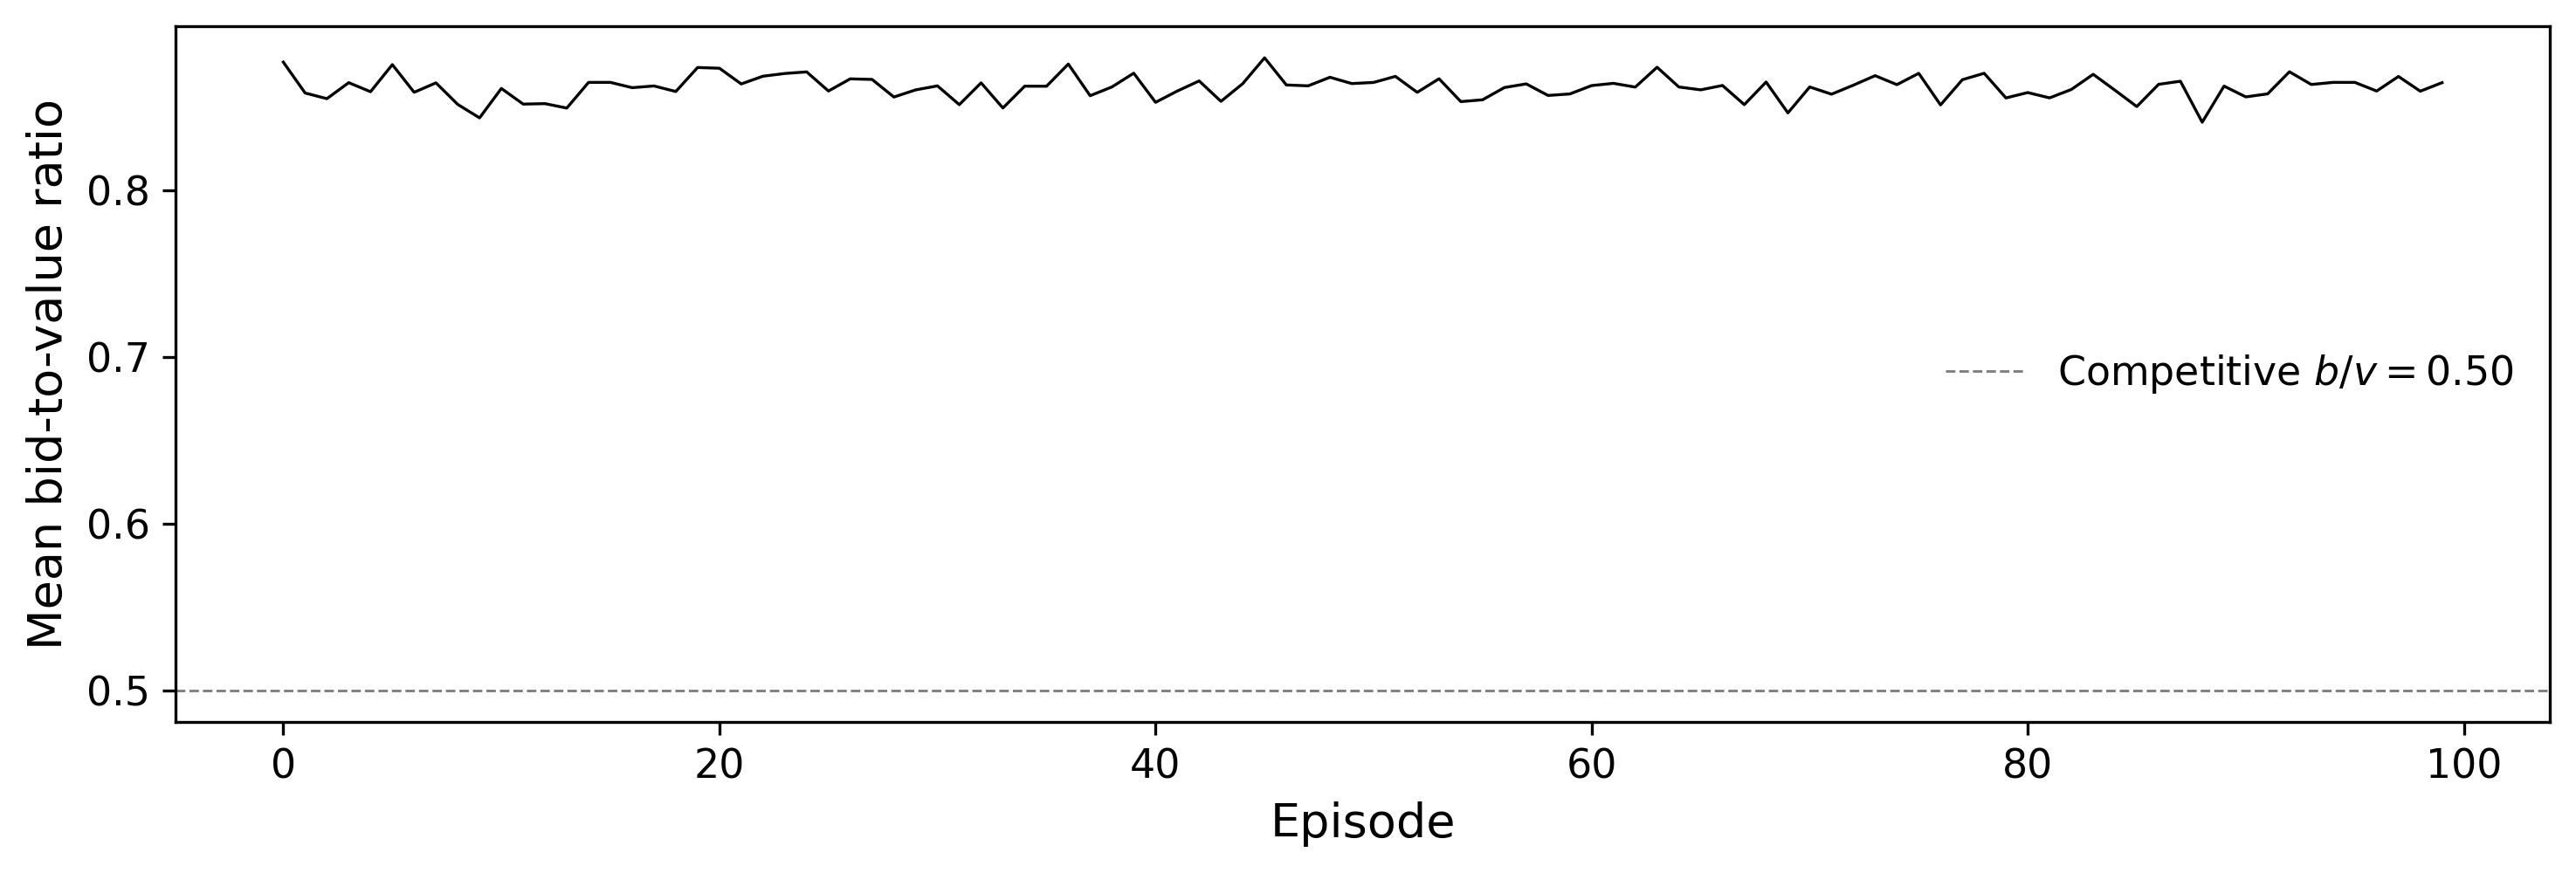
\includegraphics[width=\textwidth]{figures/e4a_trace}
  \caption{Representative learning trajectory for a single trial of Experiment~4a (first-price auction, value-maximizer objective, 2~bidders, 100 episodes $\times$ 1{,}000 rounds). Mean bid-to-value ratio per episode with the competitive benchmark (unconstrained Nash equilibrium $b/v = 0.5$).}
  \label{fig:e4a_trace}
\end{figure}

\subsection{Efficiency and Welfare}

Each episode produces a realised allocation and payments. Platform revenue is the total payments collected per episode. Liquid welfare follows Gaitonde et al.\ (2023): $W(x) = \sum_i \min(B_i, \sum_t x_{it} v_{it})$, capping each bidder's contribution at their budget. The effective Price of Anarchy divides the LP-relaxed offline optimum by realised liquid welfare: values are at least~1, with values closer to~1 indicating higher efficiency.\footnote{The LP maximises $\sum_{t,i} v_{ti} x_{ti}$ subject to $\sum_i x_{ti} \le 1$ per round and $\sum_t v_{ti} x_{ti} \le B_i$ per bidder, with fractional allocations. A greedy integer allocation provides a tighter benchmark. We report the LP-based version as the more conservative test.} Tables~\ref{tab:exp4a_ranked_rev} and~\ref{tab:exp4a_ranked_poa} report the ranked significant effects.

\input{tables/exp4a_ranked_rev}

\begin{figure}[H]
  \centering
  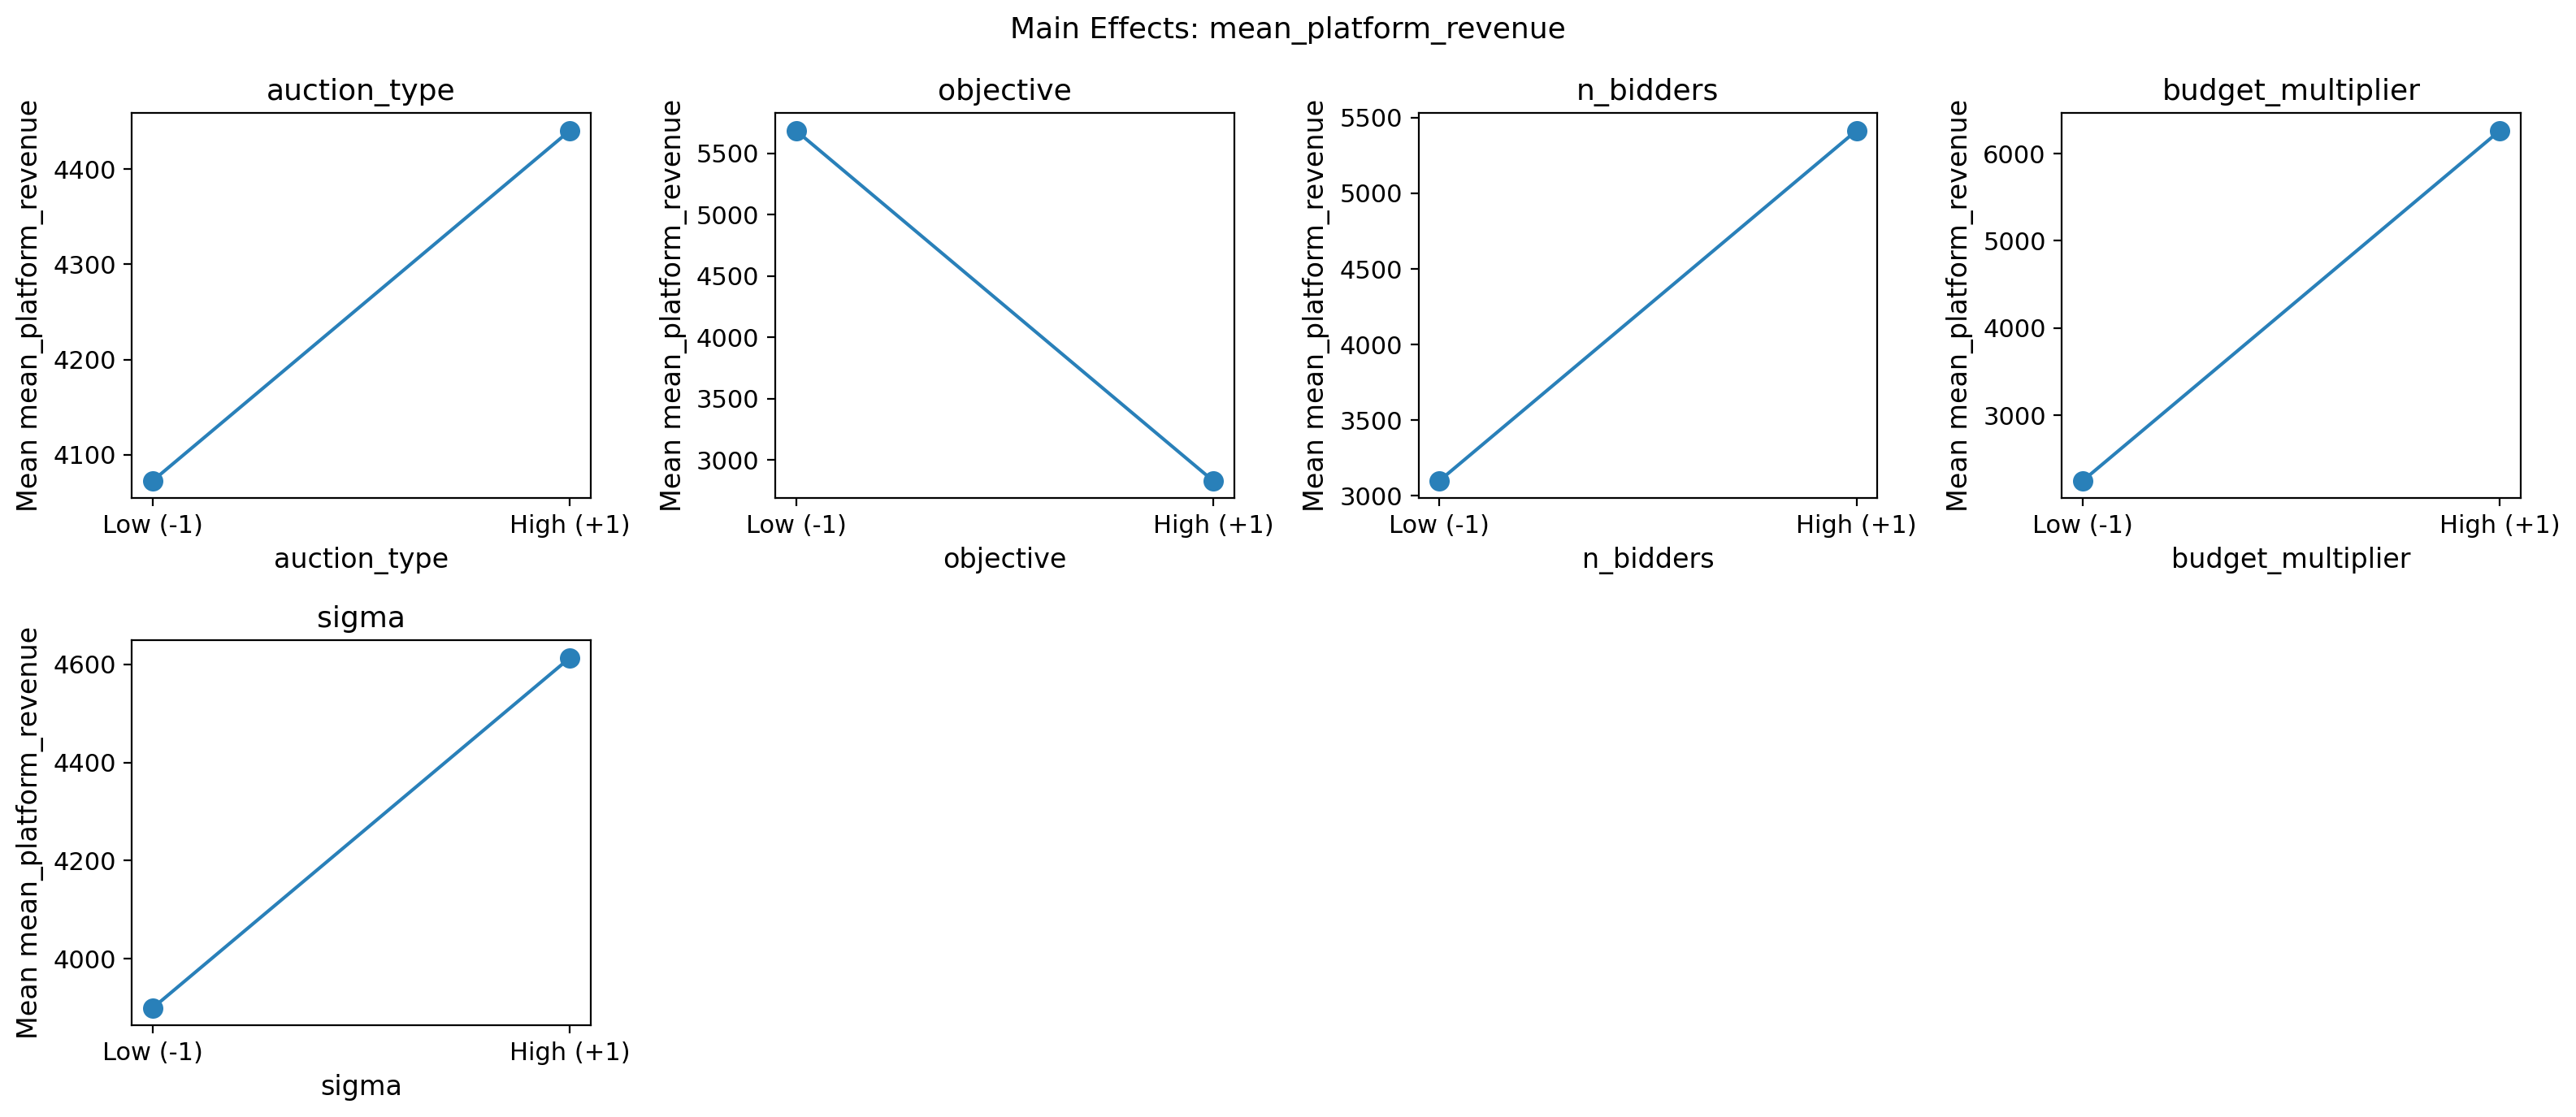
\includegraphics[width=0.7\textwidth]{figures/e4a_main_rev}
  \caption{Experiment~4a: Main effects plot for platform revenue across the three factors.}
  \label{fig:e4a_main_rev}
\end{figure}

\input{tables/exp4a_ranked_poa}

\begin{figure}[H]
  \centering
  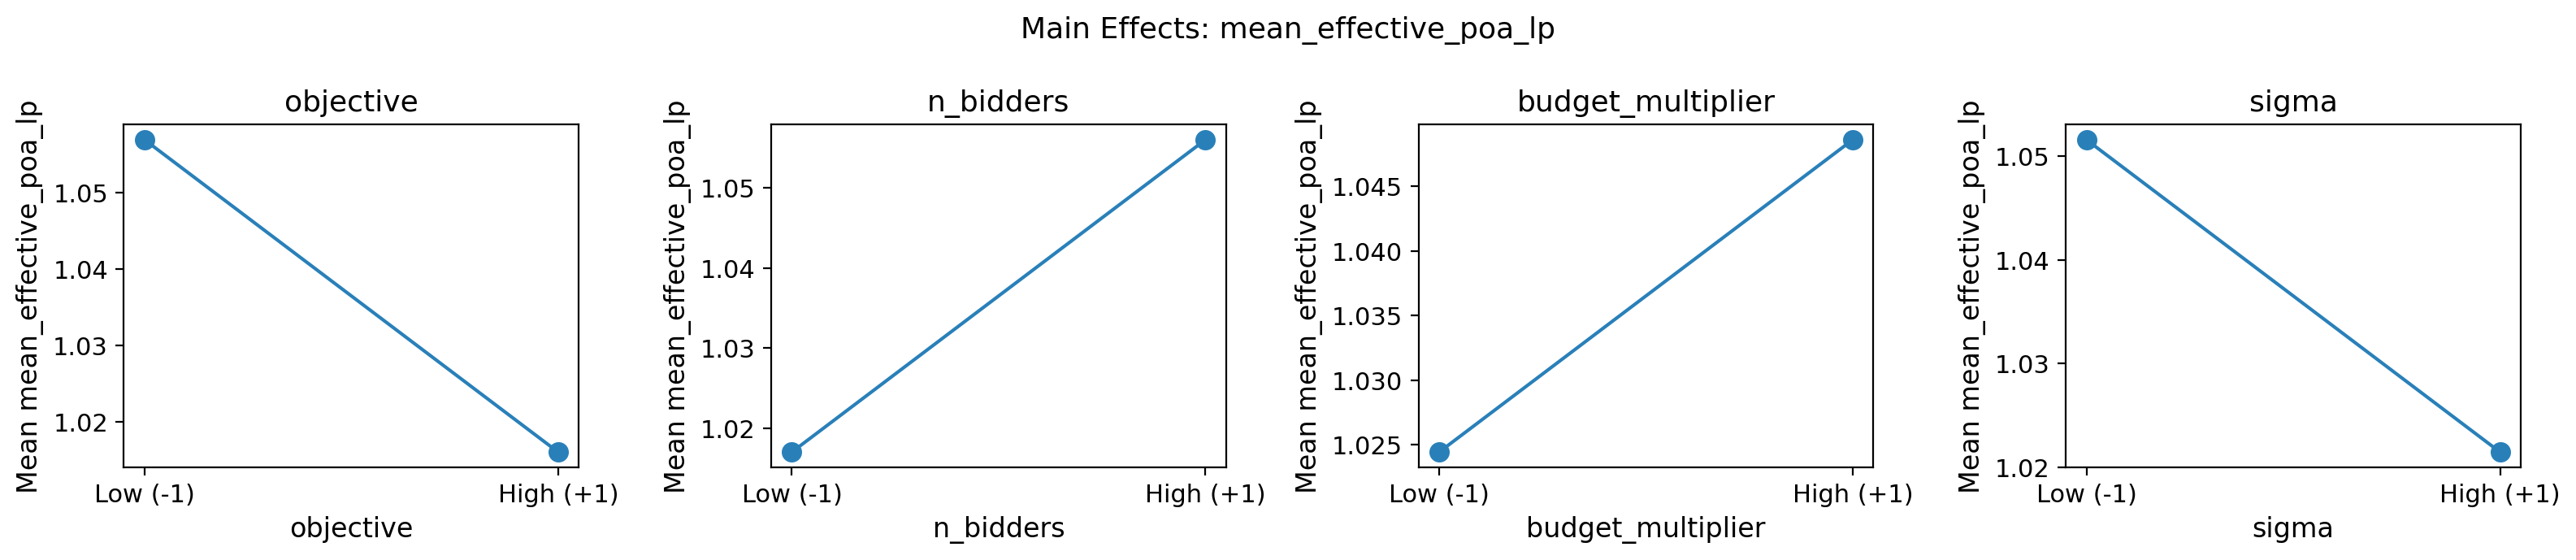
\includegraphics[width=0.7\textwidth]{figures/e4a_main_poa}
  \caption{Experiment~4a: Main effects plot for effective Price of Anarchy.}
  \label{fig:e4a_main_poa}
\end{figure}

All observed PoA values are well within the theoretical bound of~2 (Aggarwal et al.\ 2019; Gaitonde et al.\ 2023). The absence of a significant auction format effect on PoA contrasts with the revenue results: bid suppression under first-price reduces payments to the auctioneer without proportionally distorting allocative outcomes. Allocative efficiency, the fraction of rounds in which the highest-value bidder wins, provides a complementary view. Under utility-maximizing objectives, agents achieve near-perfect efficiency, because the utility-maximizing bid formula preserves relative value rankings. Under value-maximizing objectives with four bidders, efficiency drops substantially: aggressive overbidding causes frequent misallocation, as the highest bidder is not necessarily the highest-value bidder when agents bid multiples of their values.\footnote{Utility-maximizing efficiency ranges from \ExpFourAUtilEffLow{} to \ExpFourAUtilEffHigh{} across cells; value-maximizing four-bidder efficiency drops to \ExpFourAValFourEffLow--\ExpFourAValFourEffHigh, with bid-to-value ratios exceeding 1.5.} The objective$\times$n\_bidders interaction ($t = \ExpFourAAllocEffObjxNbidT$, $p \ExpFourAAllocEffObjxNbidPFmt$) captures this pattern, with more bidders amplifying the efficiency cost of value-maximizing objectives.

\subsection{Revenue and Budget Dynamics}

The budget multiplier dominates platform revenue ($|t| = \ExpFourARevFactorTOne$), shifting revenue by \ExpFourARevTopPctEffect\% of the grand mean. The number of bidders ranks fourth ($|t| = \ExpFourARevNbidAbsT$) and auction format fifth ($|t| = \ExpFourARevAuctionT$). Table~\ref{tab:exp4a_ranked_rev} reports the full hierarchy. The interaction plot (Figure~\ref{fig:e4a_int_rev}) reveals how factor combinations jointly shape revenue outcomes: market thickness interacts with auction format because additional bidders intensify competition differently under the two payment rules.

\begin{figure}[H]
  \centering
  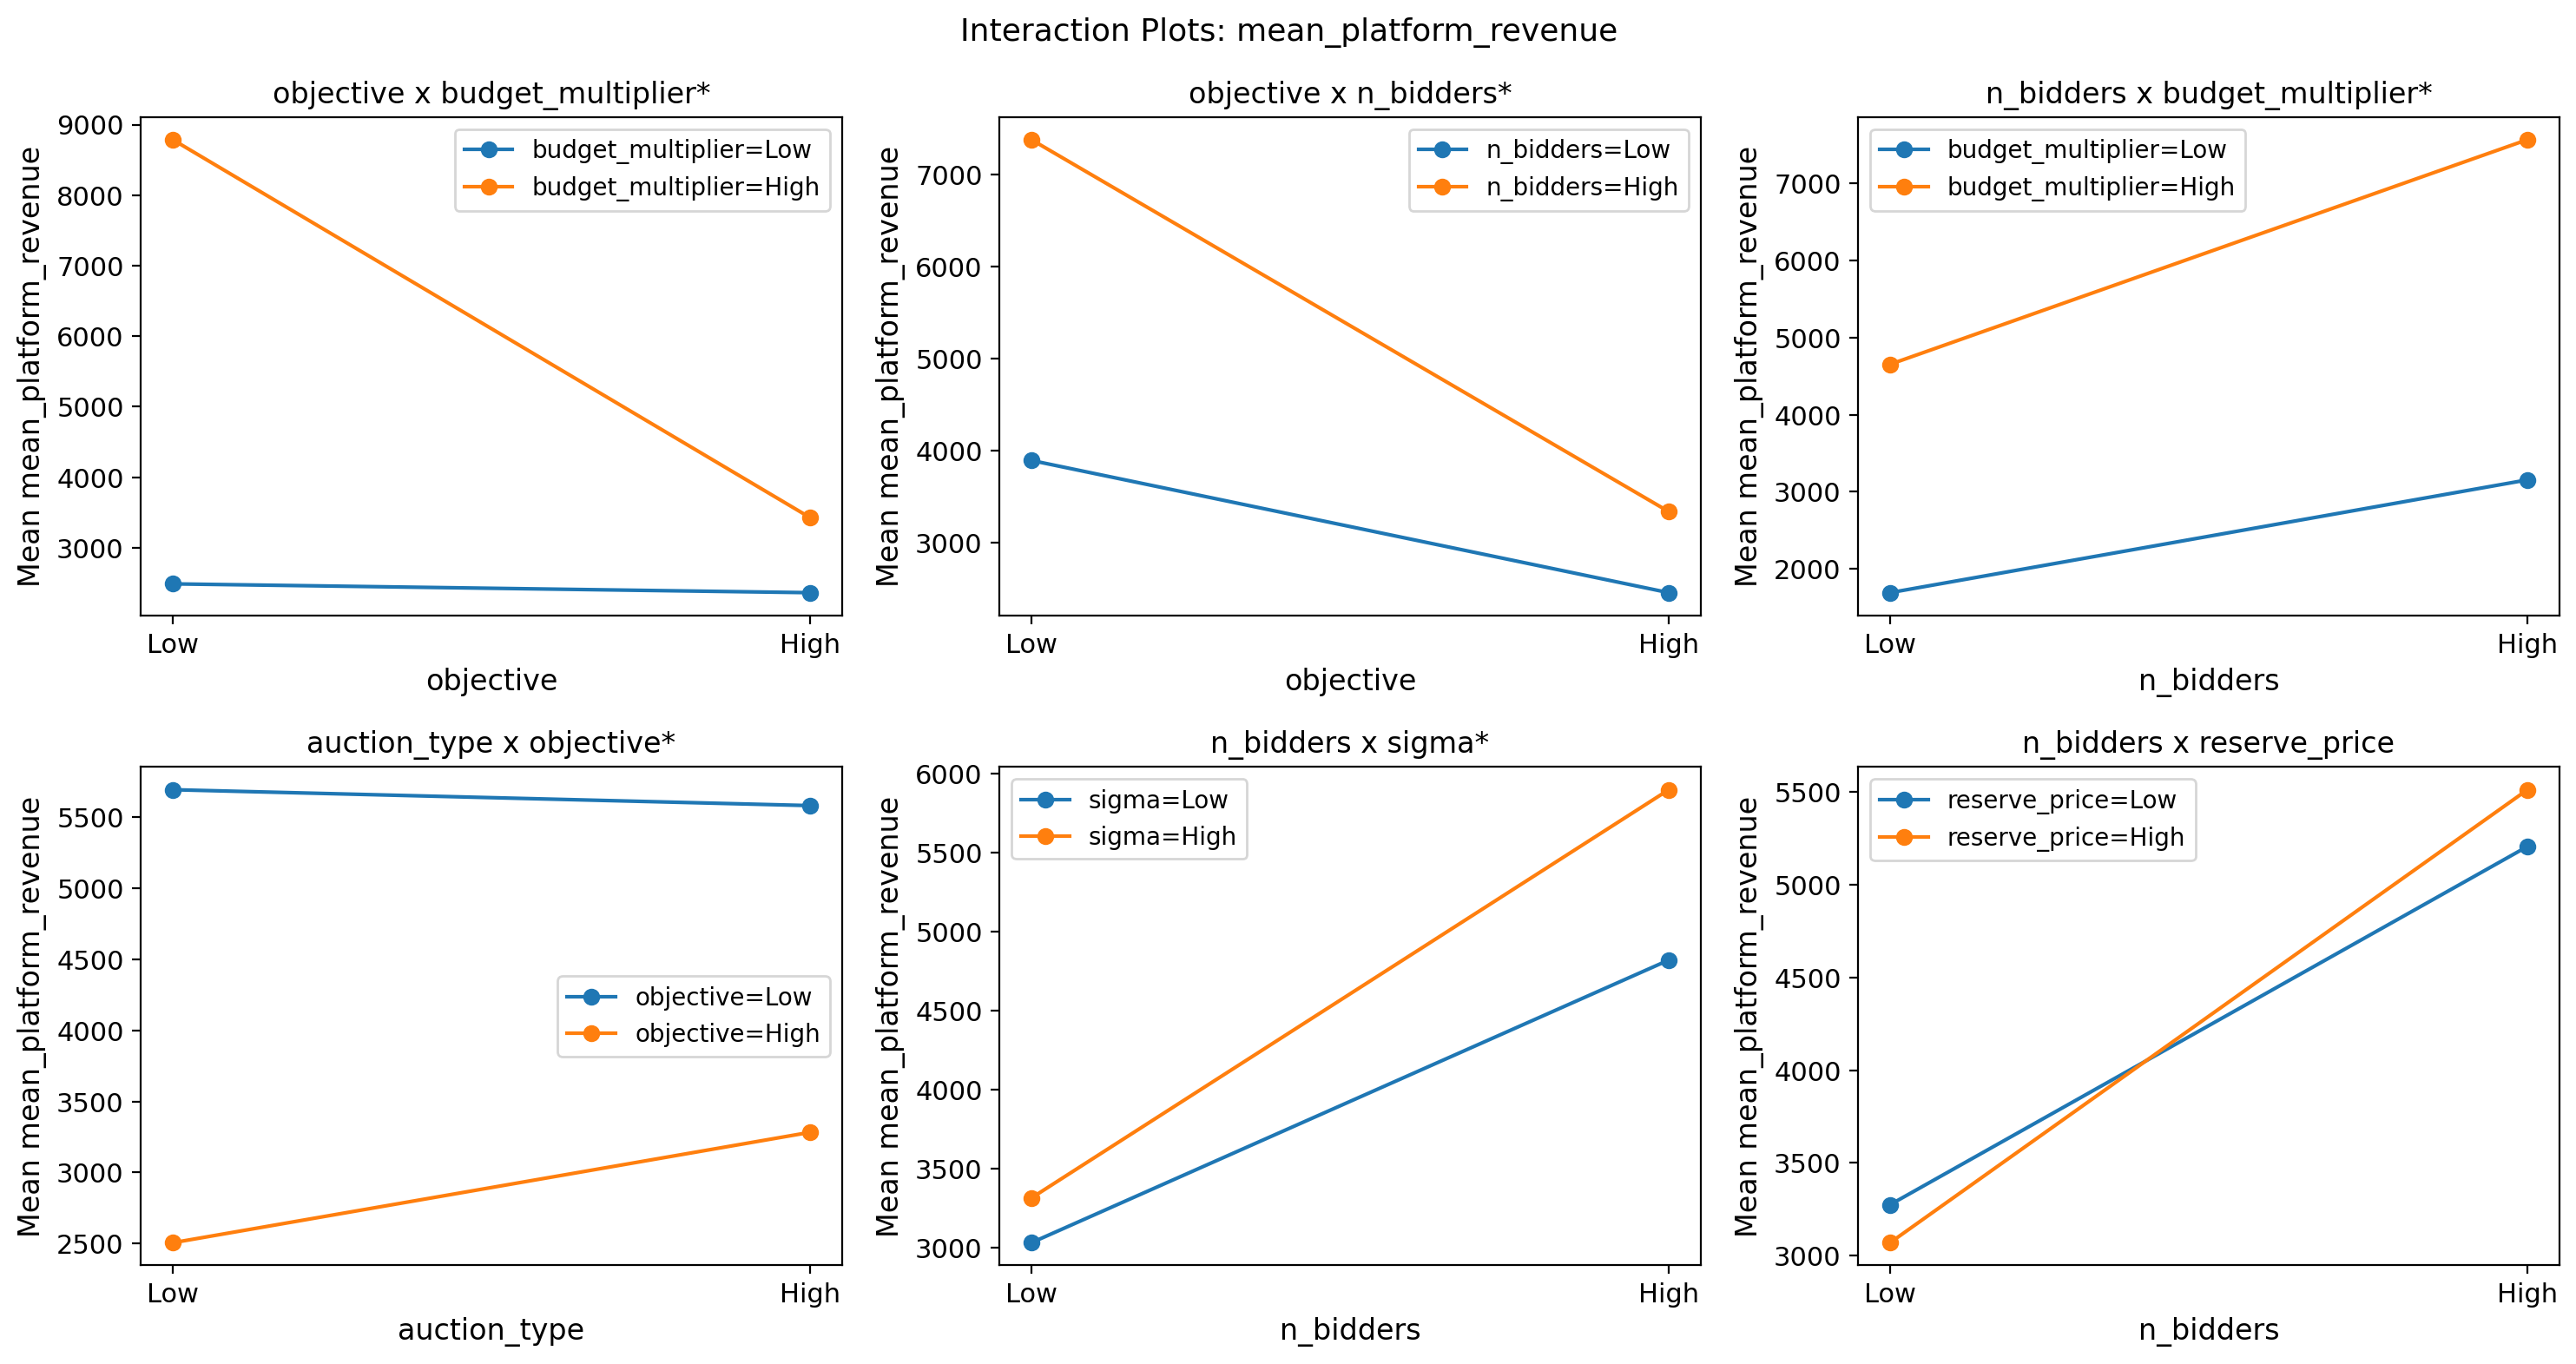
\includegraphics[width=0.7\textwidth]{figures/e4a_int_rev}
  \caption{Experiment~4a: Interaction plot for platform revenue.}
  \label{fig:e4a_int_rev}
\end{figure}

\subsection{Bidding Behaviour and Bid Suppression Indicators}

\input{tables/exp4a_ranked_vol}

\begin{figure}[H]
  \centering
  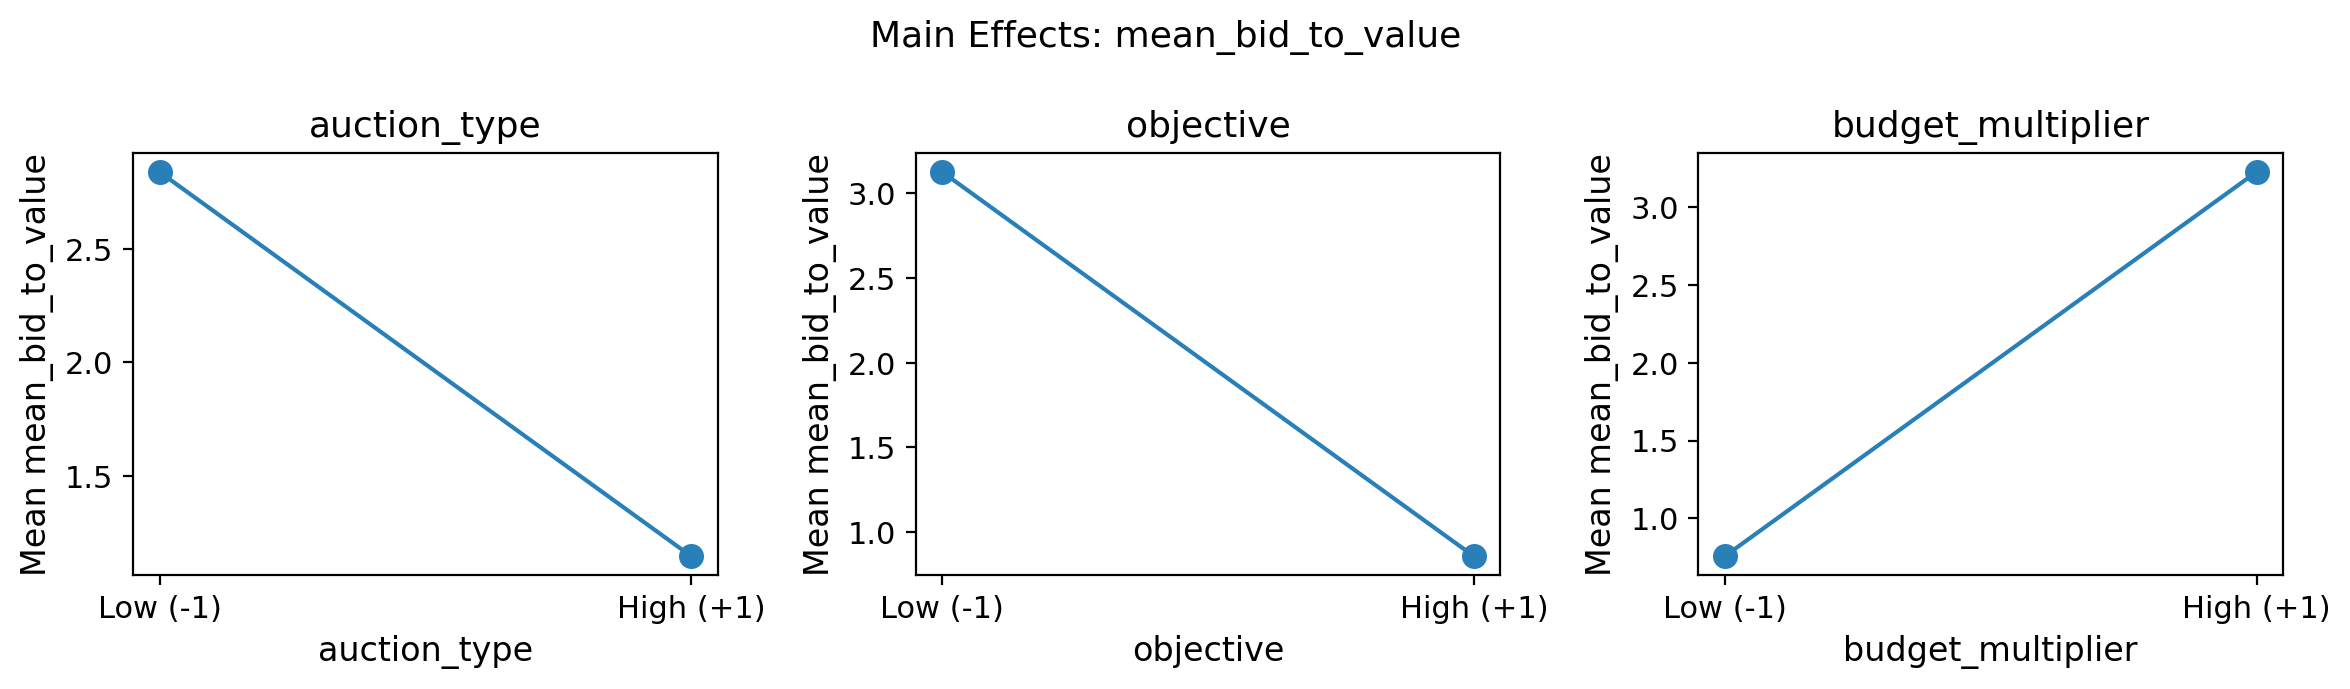
\includegraphics[width=0.7\textwidth]{figures/e4a_main_vol}
  \caption{Experiment~4a: Main effects plot for bid-to-value ratio.}
  \label{fig:e4a_main_vol}
\end{figure}

The factorial model explains \ExpFourAWelfareRsqPct\% of the variance in liquid welfare but only \ExpFourADriftRsqPct\% in cross-episode drift, reflecting substantial seed-level noise in the latter metric. Cross-episode drift, measured as the slope of the bid-to-value ratio across post-burn-in episodes, tests whether agents progressively learn to suppress bids over repeated campaign cycles, as predicted by the complex non-equilibrium dynamics of Paes Leme et al.\ (2024). Although the factorial ANOVA for drift is statistically significant ($F$-test $p \ExpFourADriftFPFmt$), the model explains only \ExpFourADriftRsqPct\% of the variance ($R^2 = \ExpFourADriftRsq$), and all cell-level drift estimates remain near zero.\footnote{The statistical significance with low $R^2$ reflects the large sample size (\ExpFourANobs{} runs) detecting economically negligible effects.} This near-zero, non-significant drift contrasts with the temporal dynamics observed in Q-learning (Experiment~2), where convergence times span tens of thousands of episodes, and suggests that dual-based pacing settles rapidly into a stable regime that does not deteriorate over repeated campaigns.

\subsection{Learning Dynamics}

Warm-start benefits are dominated by bidder objective ($t = \ExpFourAWarmObjT$): utility-maximizing agents gain substantially from retaining dual variables across episodes, while value-maximizing agents converge nearly instantly. Inter-episode volatility is similarly dominated by objective ($t = \ExpFourAIEVolObjT$), with utility-maximizing agents exhibiting higher volatility. Model adequacy diagnostics (Online Appendix~D) confirm clean inference.\footnote{$R^2$ ranges from \ExpFourARsqMin{} to \ExpFourARsqMax, PRESS gaps are below \ExpFourAPRESSGapMax, and \ExpFourABHPct\% of significant effects survive Benjamini--Hochberg correction.}

\subsection{Summary}

The budget multiplier dominates revenue (\ExpFourARevFactorOne{}, $|t| = \ExpFourARevFactorTOne$), with bidder objective ranking second and their interaction third. The number of bidders ranks fourth ($|t| = \ExpFourARevNbidAbsT$), and auction format is a comparatively minor factor ($|t| = \ExpFourARevAuctionT$). All PoA values fall well within the theoretical worst-case bound of~2.
